Design an algorithm to solve the sliding puzzle.

A \texttt{State} of this puzzle is some permutation of the puzzle tiles. There are two things we can do with a \texttt{State}:
\begin{itemize}
\item Get the set of next possible states from the current \texttt{State}.
\item Find out if the \texttt{State} is a goal: in this case when the puzzle is solved.
\end{itemize}

Imagine a game graph as a graph of all possible states where each state is a graph node and where a method, \texttt{getNextStates}, returns the neighbor nodes.
Finding a solution is equivalent to finding a path from some start state to goal state.

\marginpar{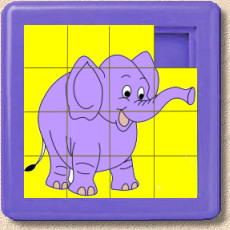
\includegraphics[width=\marginparwidth]{elephant-puzzle}}